\documentclass[10pt]{article}
\usepackage[a4paper,margin=1.5cm,top=1.2cm,bottom=1.2cm]{geometry}
\usepackage{amsmath,amssymb,graphicx,booktabs,microtype,xcolor,float}
\usepackage[T1]{fontenc}
\usepackage{lmodern}
\usepackage[font=small,labelfont=bf,skip=4pt]{caption}
\usepackage{enumitem}
\setlist{itemsep=1pt,topsep=2pt,leftmargin=1.3em}
\setlength{\parindent}{0pt}\setlength{\parskip}{4pt}
\usepackage{titlesec}
\titlespacing*{\section}{0pt}{6pt}{2pt}
\titleformat{\section}{\large\bfseries\color{black!80!blue}}{\thesection}{0.6em}{}
\newcommand{\amin}{$'$}
\pagestyle{empty}
\renewcommand{\arraystretch}{1.15}
\begin{document}

{\LARGE\bfseries Close pairs and blending of SZ clusters}\\[3pt]
{\large Two questions, answered with full-sky simulations}

\medskip
\fcolorbox{black!25}{black!4}{\begin{minipage}{0.97\textwidth}
\textbf{In short}
\begin{itemize}
\item \textbf{Close pairs are simple.} The number of clusters in an aperture follows Poisson statistics. It depends only on how many clusters there are per square degree and on the aperture's area.
\item \textbf{Detected clusters rarely sit together.} At signal-to-noise $>5$, only 0.7\% of detections have another detection within 2\amin.
\item \textbf{Blending is common anyway.} About 15\% of detections have their SZ signal inflated by more than 10\%. The culprit is many faint, undetected clusters at other redshifts along the same line of sight.
\item \textbf{So blending is a confusion problem, not a pair problem.} It must be computed from the \emph{summed} signal of all faint neighbours.
\end{itemize}
\end{minipage}}

\section{What we simulated}
We drew every galaxy cluster in the Universe above $10^{13}\,M_\odot$ out to redshift 3, using the Tinker mass function. Clusters were placed at random positions on the full sky, about 29 million of them. Each was given an SZ signal from the Planck mass--signal relation, with realistic scatter. We then ``observed'' them with an SO-like telescope: a 1.4\amin\ beam and uniform noise. A cluster counts as detected if its signal-to-noise $q$ exceeds a threshold $q_{\rm cut}$. At $q_{\rm cut}=5$ we detect 86\,000 clusters, about \textbf{2 per square degree}.

\section{Question 1: how likely are two or more clusters in one aperture?}
Clusters are placed independently, so any subset of them is also placed independently: detected clusters, massive halos, or clusters in a redshift slice. The number $N$ inside an aperture of radius $\theta$ then follows a Poisson law:
\[
P(N=n)=\frac{e^{-\mu}\,\mu^n}{n!},\qquad \mu=\Sigma\times\pi\theta^2 ,
\]
where $\Sigma$ is the number of clusters of the chosen kind per unit area.
\begin{itemize}
\item \textbf{Around a detected cluster} the same formula gives the number of \emph{other} clusters. The chance of at least one neighbour is $1-e^{-\mu}\approx\mu$.
\item \textbf{Over the whole sky} the expected number of close pairs is $N_{\rm total}\,\mu/2$.
\end{itemize}

\begin{figure}[H]
\centering
\begin{minipage}[c]{0.31\textwidth}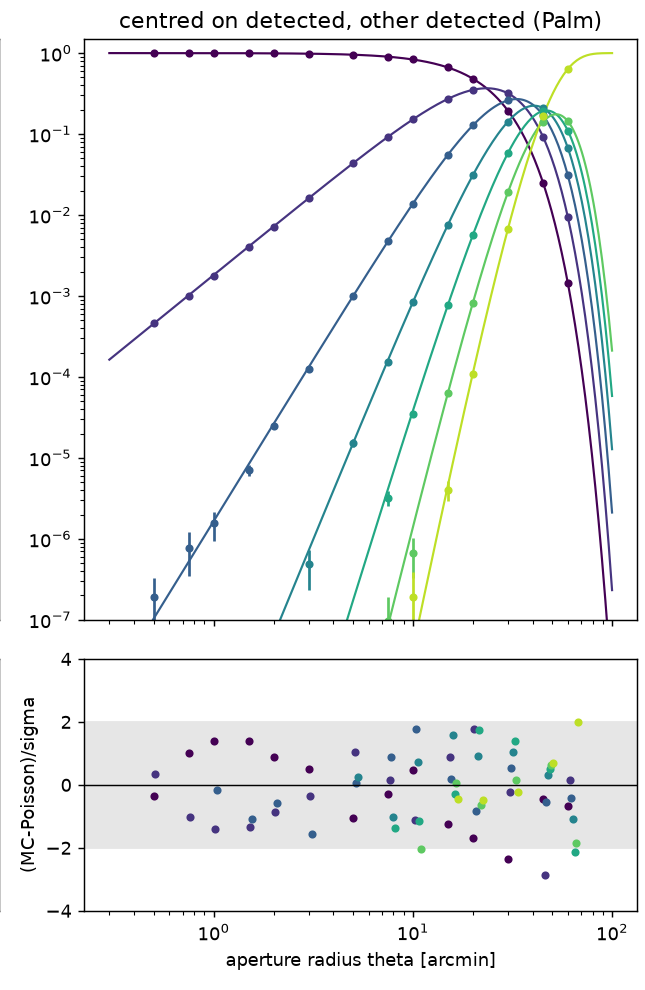
\includegraphics[width=\linewidth]{f1p.png}\end{minipage}\hfill
\begin{minipage}[c]{0.64\textwidth}
\small
\begin{tabular}{@{}lcccc@{}}
\toprule
\multicolumn{5}{@{}l}{\textbf{Chance that a detected cluster ($q>5$) has a neighbour}}\\
neighbour within & 1\amin & 2\amin & 5\amin & 10\amin\\
\midrule
another detected cluster & 0.2\% & 0.7\% & 4\% & 17\%\\
any halo $>10^{14}M_\odot$ & 0.8\% & 3\% & 19\% & 57\%\\
any halo $>3\times10^{13}M_\odot$ & 9\% & 32\% & 91\% & 100\%\\
\midrule
close pairs of detections, full sky & 78 & 312 & 1950 & 7800\\
\bottomrule
\end{tabular}
\captionof{figure}{Left: the probability of finding $n$ other detected clusters within radius $\theta$ of a detected cluster. Dots are 120 simulated skies; lines are the Poisson formula, with nothing fitted. Colours run from $n=0$ (dark) to $n\ge6$ (yellow). They agree everywhere.}
\end{minipage}
\end{figure}

\textbf{Caveat.} Real clusters are clustered, and these simulated ones are not. Clustering raises close-pair probabilities by about 15--25\% at 1--5\amin. To include it, multiply $\mu$ by that factor.

\clearpage
\section{Question 2: how often is a detection blended?}
Neighbours can affect a detection in four ways:

\begin{center}\small
\begin{tabular}{@{}lp{0.72\textwidth}@{}}
\toprule
\textbf{Merged pair} & two clusters that would each be detected are so close that the pipeline sees only one\\
\textbf{Contaminated} & a real detection whose signal (and so mass) is inflated by neighbours\\
\textbf{Boosted} & a cluster too faint to be detected alone, pushed over the threshold by neighbours\\
\textbf{Lost} & a cluster detectable alone that is missed: swallowed by a brighter peak, or pulled below threshold\\
\bottomrule
\end{tabular}
\end{center}

We measured these in two independent ways. One is a calculation from the catalogue, described below. The other is a set of simulated maps covering 32\,000 deg$^2$, with every halo painted in, noise added and a real detection pipeline run.

\begin{figure}[H]
\centering
\begin{minipage}[c]{0.36\textwidth}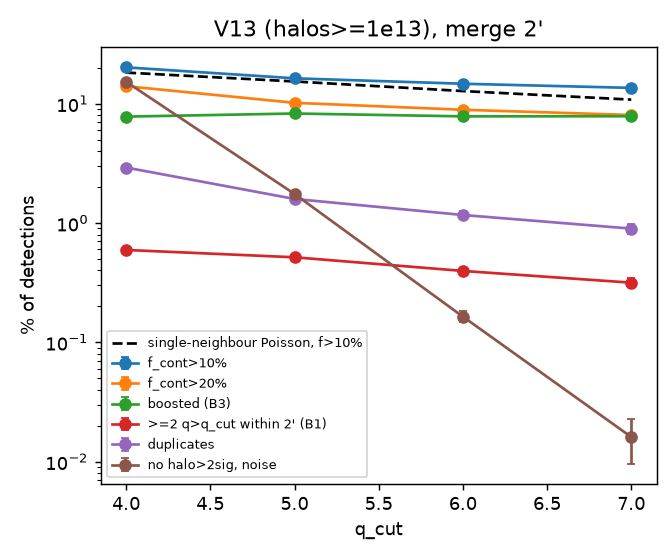
\includegraphics[width=\linewidth]{f2b.png}\end{minipage}\hfill
\begin{minipage}[c]{0.61\textwidth}
\small
\begin{tabular}{@{}lcccc@{}}
\toprule
threshold $q_{\rm cut}$ & 4 & 5 & 6 & 7\\
\midrule
merged pairs & 0.6\% & 0.5\% & 0.4\% & 0.3\%\\
contaminated by $>10\%$ & 14--19\% & 14--16\% & 14--15\% & 13\%\\
contaminated by $>20\%$ & 8--12\% & 8--11\% & 8--9\% & 7--8\%\\
boosted & 8--9\% & 8\% & 8\% & 7--8\%\\
lost & 11--12\% & 9--10\% & 8--9\% & 7--8\%\\
\bottomrule
\end{tabular}
\captionof{figure}{Table: ranges span the catalogue calculation and the maps. Lost is a percentage of clusters detectable on their own; other rows are percentages of detections. Left: map results. Merged pairs (red) stay below 1\%; contamination and boosting (blue, orange, green) are 15--30 times larger. Brown: pure-noise peaks.}
\end{minipage}
\end{figure}

\textbf{Why pairs are the wrong picture.} Each cluster sits on a background of many faint halos. Each one is too faint to see, but together they add a sizeable, fluctuating signal. Most of this extra signal comes from halos around $10^{14}\,M_\odot$ at other redshifts. No single ``blending radius'' describes it: the radius you would need grows from 8\amin\ to 12\amin\ as the threshold rises.

\textbf{How to compute it.} Use the method radio astronomers use for source confusion (``P(D)''):
\begin{enumerate}[itemsep=1pt]
\item Every halo near the cluster adds signal, weighted by the filter's response at that distance.
\item The halos are random (Poisson), so the distribution of the total added signal follows directly from the mass function. One Fourier transform computes it.
\item Add the noise, apply the threshold, and count how often the added signal matters.
\end{enumerate}
This calculation reproduces the simulated maps to within about 2 percentage points.

\textbf{Two traps.}
\begin{itemize}
\item \textbf{Remove the mean SZ signal of the map.} The faint halos give the whole sky a small average signal. A plain matched filter reads that as extra signal from the cluster. If it is not subtracted, every blending fraction roughly triples.
\item \textbf{Count on the detected sample.} Clusters that received extra signal are more likely to pass the cut. Blending among \emph{detected} clusters is therefore 1.3--1.5 times higher than a naive estimate.
\end{itemize}

\section{How robust is this?}
\begin{itemize}
\item \textbf{Close pairs (Q1)} stay exactly Poisson for every noise level, beam and mass function we tried. Only the number of detections per square degree changes.
\item \textbf{Blending fractions} rise by about 1.3--1.4 times with half the noise or a 5\amin\ beam. They change by under 10\% with a different mass function, different scatter or clustering.
\item \textbf{Physical overlap} of clusters in 3D accounts for only 0.1\% of close pairs. Blending is a projection effect.
\end{itemize}

\section{Conclusions}
\begin{itemize}
\item \textbf{To predict close pairs}, use Poisson statistics with $\mu=\Sigma\pi\theta^2$, plus about 20\% for clustering at arcminute scales.
\item \textbf{To predict blending}, do not count pairs. Compute the summed signal of all halos down to $10^{13}\,M_\odot$, remove the map mean, and measure fractions on the detected sample. Check once with your own pipeline on maps.
\item \textbf{Expect, for an SO-like survey at $q>5$:} 0.5\% merged pairs, about 15\% of detections contaminated by more than 10\%, about 8\% boosted over the threshold, and about 10\% of real clusters lost.
\end{itemize}
\end{document}
